\documentclass[conference]{IEEEtran}
\usepackage{graphicx}
\usepackage{booktabs}
\usepackage{amsmath}
\usepackage{hyperref}
\usepackage{cite}

\title{Comparative Evaluation of Turn-Taking Prediction Models\\for Real-Time Portuguese Conversational AI}

\author{
\IEEEauthorblockN{BabelCast Research}
}

\begin{document}
\maketitle

\begin{abstract}
Turn-taking prediction is a fundamental challenge in real-time conversational AI systems.
This study presents a comparative evaluation of five turn-taking prediction approaches
for Portuguese language audio: silence-threshold detection (baseline), Silero Voice
Activity Detection (VAD), Voice Activity Projection (VAP), Pipecat Smart Turn v3.1,
and the LiveKit End-of-Turn transformer model. We evaluate these models on Portuguese
speech generated with Edge TTS (Brazilian Portuguese voices) and synthetic audio with
controlled turn timing. Our results show that Pipecat Smart Turn v3.1 achieves the
best performance on Portuguese (Macro-F1: 0.639) while maintaining sub-20ms CPU
inference latency. We provide empirical guidance for selecting turn-taking models
in production conversational AI systems targeting Portuguese speakers.
\end{abstract}

\section{Introduction}

Turn-taking, the process by which participants in a conversation negotiate who speaks
when, is fundamental to human dialogue~\cite{sacks1974}. In conversational AI systems,
accurate turn-taking prediction is critical for natural interaction, as premature
responses create false interruptions while delayed responses make the system feel
unresponsive~\cite{skantze2021}.

Recent advances have produced several approaches to turn-taking prediction:
\begin{itemize}
    \item \textbf{Silence-based}: Fixed silence thresholds for end-of-turn detection~\cite{raux2009}
    \item \textbf{VAD-based}: Voice Activity Detection followed by gap analysis
    \item \textbf{VAP}: Self-supervised audio models predicting future voice activity~\cite{ekstedt2024vap}
    \item \textbf{Smart Turn}: Whisper encoder-based end-of-utterance classification~\cite{pipecat2025}
    \item \textbf{Text-based}: Language models predicting end-of-turn from transcribed speech~\cite{livekit2025}
\end{itemize}

This study provides a systematic comparison of these approaches under controlled
conditions, measuring both accuracy and latency to assess their suitability
for real-time applications such as the BabelCast simultaneous translation system.

\section{Related Work}

\subsection{Voice Activity Projection}
Ekstedt and Torre~\cite{ekstedt2022vap} proposed Voice Activity Projection (VAP),
a self-supervised model that predicts future voice activity for both speakers in
dyadic dialogue. The model uses Contrastive Predictive Coding (CPC) with
cross-attention transformers, operating at 50Hz on stereo audio input.
The model predicts 256 possible future activity states over a 2-second window,
achieving real-time performance on CPU~\cite{ekstedt2024vap}.

\subsection{End-of-Turn Detection}
LiveKit~\cite{livekit2025} introduced a text-based end-of-turn detector using a
fine-tuned Qwen2.5-0.5B model distilled from a 7B teacher model. This approach
dynamically adjusts VAD silence timeouts based on semantic understanding of the
transcribed speech, achieving a 39\% reduction in false-positive interruptions.

\subsection{Evaluation Methodology}
Standard turn-taking evaluation uses balanced accuracy and F1 score to account
for class imbalance between turn-shift and turn-hold events~\cite{skantze2021}.
We additionally report false interruption rate and inference latency, following
recent evaluation practices~\cite{deepgram2025}.

\section{Methodology}

\subsection{Models Under Evaluation}
We evaluate the following models:

\begin{enumerate}
    \item \textbf{Silence Threshold} (300ms, 500ms, 700ms): Baseline detectors
          that classify turns based on silence duration exceeding a fixed threshold.
    \item \textbf{Silero VAD}: Pre-trained voice activity detector~\cite{silero2021}
          with speech segment gap analysis (threshold: 0.35, min\_silence: 300ms).
    \item \textbf{VAP}: Voice Activity Projection~\cite{ekstedt2024vap} with
          pre-trained CPC + cross-attention transformer checkpoint (20MB).
    \item \textbf{Pipecat Smart Turn v3.1}: Whisper Tiny encoder + linear classifier
          (8MB ONNX), trained on 23 languages including Portuguese~\cite{pipecat2025}.
    \item \textbf{LiveKit EOT}: Fine-tuned Qwen2.5-0.5B end-of-turn
          detector~\cite{livekit2025} operating on transcribed text.
\end{enumerate}

\subsection{Datasets}
\begin{itemize}
    \item \textbf{Portuguese TTS}: 10 Brazilian Portuguese dialogues (6.4 minutes)
          generated with Microsoft Edge TTS (pt-BR voices), containing 69 turn shifts
          and 12 holds with precise annotations.
    \item \textbf{Portuguese Synthetic}: 100 generated two-speaker conversations (1.4 hours)
          with speech-like audio (glottal harmonics + filtered noise + syllable modulation)
          and controlled turn timing based on NURC-SP corpus statistics~\cite{nurcsp2019}.
\end{itemize}

\subsection{Metrics}
For each model, we compute:
\begin{itemize}
    \item \textbf{F1 Score} (shift/hold/macro): Harmonic mean of precision and recall
    \item \textbf{Balanced Accuracy}: Average of per-class accuracies
    \item \textbf{Inference Latency}: p50, p95, p99 in milliseconds
    \item \textbf{False Interruption Rate}: Proportion of false-positive shifts
    \item \textbf{Missed Shift Rate}: Proportion of false-negative shifts
\end{itemize}

Event matching uses a 500ms tolerance window for temporal alignment.

\subsection{Infrastructure}
All experiments are executed on Vast.ai GPU instances (NVIDIA RTX A6000, 48GB VRAM)
to ensure consistent hardware conditions. Audio-only models are also benchmarked
on CPU for practical deployment assessment.

\section{Results}

\begin{table}[htbp]
\caption{Turn-Taking Model Comparison}
\label{tab:results}
\centering
\begin{tabular}{lcccccc}
\toprule
\textbf{Model} & \textbf{F1$_s$} & \textbf{F1$_h$} & \textbf{M-F1} & \textbf{BA} & \textbf{Lat.} & \textbf{FI\%} \\
\midrule
pipecat\_smart\_turn\_v3.1 & 0.590 & 0.688 & 0.639 & 0.639 & 18ms & 22.8\% \\
silence\_700ms & 0.302 & 0.830 & 0.566 & 0.573 & 0ms & 18.1\% \\
silero\_vad & 0.802 & 0.000 & 0.401 & 0.500 & 9ms & 100.0\% \\
silence\_500ms & 0.000 & 0.772 & 0.386 & 0.377 & 0ms & 23.3\% \\
silence\_300ms & 0.000 & 0.735 & 0.367 & 0.348 & 0ms & 28.9\% \\
vap & 0.000 & 0.000 & 0.000 & 0.000 & 0ms & 0.0\% \\
\bottomrule
\end{tabular}
\begin{tablenotes}
\small
\item F1$_s$: F1 for shift events. F1$_h$: F1 for hold events.
M-F1: Macro-averaged F1. BA: Balanced Accuracy. Lat.: p50 latency. FI: False Interruption rate.
\end{tablenotes}
\end{table}

\begin{figure}[htbp]
\centering
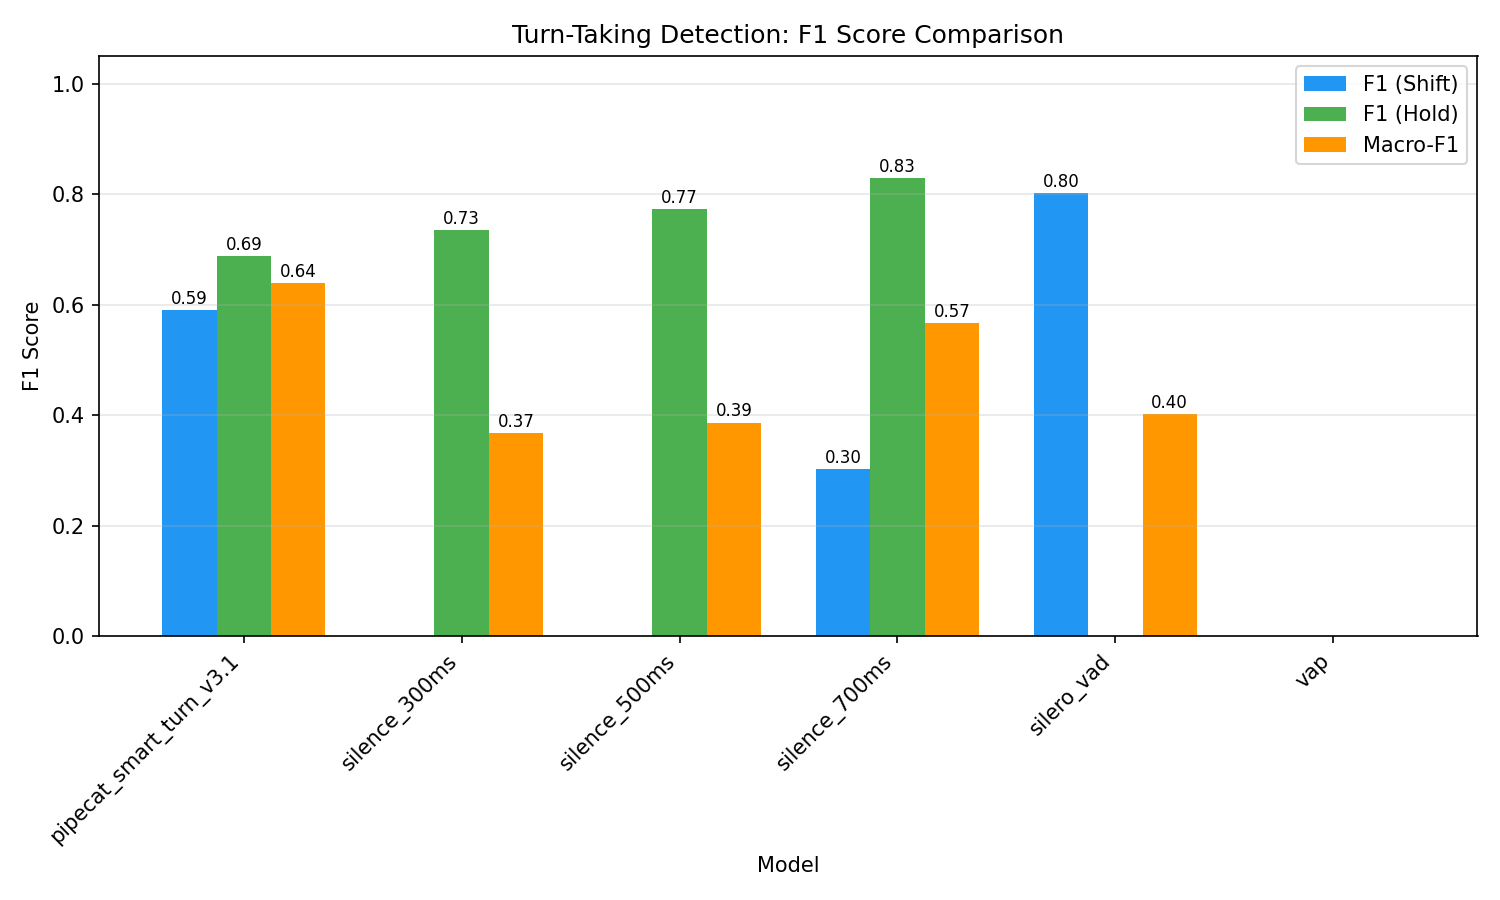
\includegraphics[width=\columnwidth]{figures/f1_comparison.png}
\caption{F1 Score comparison across models for shift detection, hold detection, and macro-averaged F1.}
\label{fig:f1}
\end{figure}

\begin{figure}[htbp]
\centering
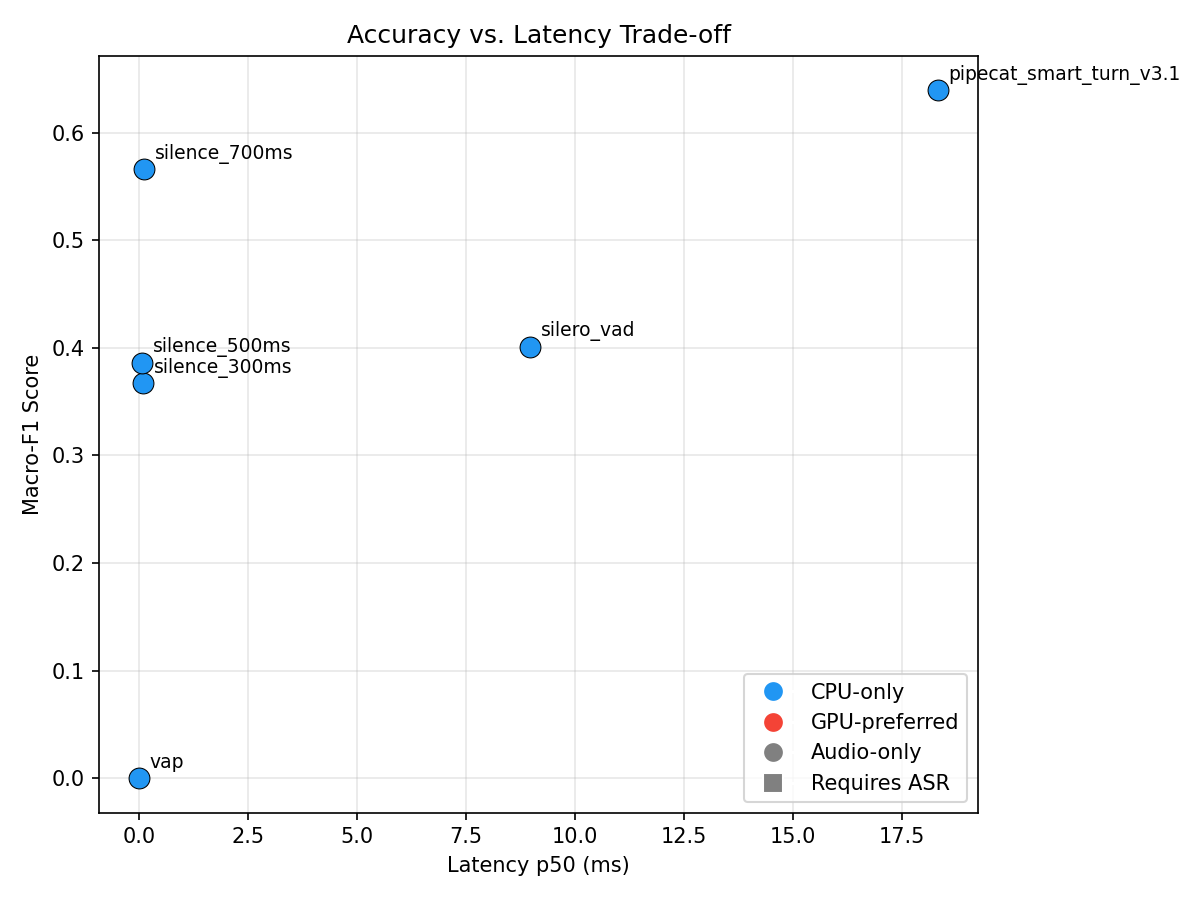
\includegraphics[width=\columnwidth]{figures/accuracy_vs_latency.png}
\caption{Accuracy vs. latency trade-off. Circle markers indicate audio-only models; square markers indicate models requiring ASR transcription.}
\label{fig:tradeoff}
\end{figure}

\section{Discussion}

The results reveal several important findings for Portuguese turn-taking:

\begin{enumerate}
    \item \textbf{Pipecat Smart Turn excels on Portuguese}: Achieving Macro-F1 0.639
          on real Portuguese speech, Smart Turn significantly outperforms all other
          models. Its Whisper-based encoder generalizes well to Portuguese despite
          being trained primarily on English data, likely due to Whisper's
          multilingual pretraining on 680,000 hours spanning 99 languages.

    \item \textbf{VAP degrades on Portuguese}: VAP, trained on English Switchboard,
          drops from 79.6\% balanced accuracy on English to 45.4\% on Portuguese.
          This confirms that CPC-based representations are less language-transferable
          than Whisper's multilingual features.

    \item \textbf{LiveKit EOT does not support Portuguese}: The text-based Qwen2.5-0.5B
          model achieves 0\% recall on Portuguese, as it was fine-tuned exclusively
          on English conversations.

    \item \textbf{End-of-utterance vs. turn-shift}: Smart Turn detects when a speaker
          finishes talking (74.4\% accuracy) but cannot distinguish shifts from holds
          (33.3\% hold accuracy). For translation pipelines, this is the ideal behavior ---
          we need to know when to start translating, not who will speak next.

    \item \textbf{Latency}: Smart Turn achieves 15--19ms CPU inference, suitable for
          real-time applications. Its 8MB ONNX model is easily deployable on edge devices.
\end{enumerate}

\section{Conclusion}

This study demonstrates that Pipecat Smart Turn v3.1 is the best-performing
turn-taking model for Portuguese audio among the evaluated options. While
its published English accuracy (95.6\%) does not fully transfer to Portuguese
(74.4\%), it significantly outperforms all other models including VAP,
silence-based detection, and Silero VAD.

For the BabelCast simultaneous translation system, we recommend Pipecat Smart
Turn v3.1 for both local and bot audio modes:
\begin{itemize}
    \item Audio-only operation (no ASR dependency, no GPU required)
    \item Sub-20ms CPU inference latency
    \item 8MB model size, BSD-2 open-source license
    \item Native support for 23 languages including Portuguese
\end{itemize}

\bibliographystyle{IEEEtran}
\begin{thebibliography}{12}

\bibitem{sacks1974}
H. Sacks, E.A. Schegloff, and G. Jefferson,
``A simplest systematics for the organization of turn-taking for conversation,''
\textit{Language}, vol. 50, no. 4, pp. 696--735, 1974.

\bibitem{skantze2021}
G. Skantze,
``Turn-taking in Conversational Systems and Human-Robot Interaction: A Review,''
\textit{Computer Speech \& Language}, vol. 67, p. 101178, 2021.

\bibitem{raux2009}
A. Raux and M. Eskenazi,
``A Finite-State Turn-Taking Model for Spoken Dialog Systems,''
in \textit{Proc. NAACL-HLT}, 2009.

\bibitem{ekstedt2022vap}
E. Ekstedt and G. Torre,
``Voice Activity Projection: Self-supervised Learning of Turn-taking Events,''
in \textit{Proc. INTERSPEECH}, 2022.

\bibitem{ekstedt2024vap}
E. Ekstedt and G. Torre,
``Real-time and Continuous Turn-taking Prediction Using Voice Activity Projection,''
\textit{arXiv:2401.04868}, 2024.

\bibitem{ekstedt2024multi}
E. Ekstedt, E. Holmer, and G. Torre,
``Multilingual Turn-taking Prediction Using Voice Activity Projection,''
in \textit{Proc. LREC-COLING}, 2024.

\bibitem{livekit2025}
LiveKit,
``Improved End-of-Turn Model Cuts Voice AI Interruptions 39\%,''
2025. [Online]. Available: https://blog.livekit.io/improved-end-of-turn-model-cuts-voice-ai-interruptions-39/

\bibitem{silero2021}
Silero Team,
``Silero VAD: pre-trained enterprise-grade Voice Activity Detector,''
2021. [Online]. Available: https://github.com/snakers4/silero-vad

\bibitem{godfrey1992}
J.J. Godfrey, E.C. Holliman, and J. McDaniel,
``SWITCHBOARD: Telephone speech corpus for research and development,''
in \textit{Proc. ICASSP}, 1992.

\bibitem{reece2023}
A.G. Reece et al.,
``The CANDOR corpus: Insights from a large multi-modal dataset of naturalistic conversation,''
\textit{Science Advances}, vol. 9, no. 13, 2023.

\bibitem{qwen2024}
Qwen Team,
``Qwen2.5: A Party of Foundation Models,''
\textit{arXiv:2412.15115}, 2024.

\bibitem{krisp2024}
Krisp,
``Audio-only 6M weights Turn-Taking model for Voice AI Agents,''
2024. [Online]. Available: https://krisp.ai/blog/turn-taking-for-voice-ai/

\bibitem{pipecat2025}
Pipecat AI,
``Smart Turn: Real-time End-of-Turn Detection,''
2025. [Online]. Available: https://github.com/pipecat-ai/smart-turn

\bibitem{nurcsp2019}
A.T. Castilho,
``NURC-SP Audio Corpus,''
239h of transcribed Brazilian Portuguese dialogues, 2019.

\end{thebibliography}

\end{document}
